\section{Results}
\label{sec:results}

\subsection{Conventions: every asset needs the same three corrections}
\label{sec:conventions}

H1 holds with one marginal exception. All 24 raw assets carry the same root
rotation, $+90^\circ$ about $X$ (the mesh is stored $Z$-up and rotated into
glTF's $Y$-up), all are double-sided, and all use the same material layout: one
primitive, one material with \texttt{KHR\_materials\_specular}, and three
4096$^2$ PNG maps (base colour, normal, metallic-roughness). Every file names
Blender's glTF exporter as its generator. Scale is normalised regardless of
subject: the largest extent is 0.895--1.151 units (median 1.082), so a camel, a
cart, a stupa and a soldier all arrive about one unit long. One asset, the
milestone, falls 0.005 below the pre-registered 0.9 bound. The pivot sits on the
base of the bounding box in every case (vertical fraction 0.000) and near, but
not at, its horizontal centre (0.30--0.69 of the depth).

None of this is a defect in itself. Feet at the origin is the convention a game
wants, and a $+90^\circ$ node is correct glTF. But two of the three corrections
the game needed for every asset cannot be derived from the file: real-world size
must come from outside, and the facing direction ($-Z$, so the character shows its
back to a player standing in front of it) is not encoded anywhere. The only
property a counting check could not see is the one that caused the first fix.

\subsection{Hygiene: the generator's meshes are clean; ours was not}
\label{sec:hygiene}

H2 is not supported. All 24 raw assets are watertight and edge-manifold, with no
degenerate or duplicate faces; 19 are a single connected component and five
consist of two to four (Wilson 95\% CI for failing any of the three checks:
9--41\%). What every asset does have is self-intersections (11--524 faces,
median 64) and a high genus (median 60, up to 361), consistent with small
tunnels in a surface extracted from an implicit field. None of these showed up
in play.

The UV layouts are where the meshes depart from hand-made assets. The 24 raw
assets have 703--3,088 UV charts each (median 1,568), and the union of their UV
triangles covers 48--68\,\% of the texture square (median 53\,\%): about half of
every 4096$^2$ map stores nothing. Charts do not overlap. Seams split vertices
1.31--1.81 times over (median 1.53), so the vertex buffer the GPU receives is half
again as large as the surface needs.

The one mesh that fails every check is the one we processed. The companion's raw
497,850-triangle file is watertight, manifold and a single component, like the
others. The shipped 82,829-triangle version has 2,433 components, 44,316 open edges
and 1,442 non-manifold vertices; welding at tolerances up to $10^{-4}$ of the
diagonal closes none of them. Section~\ref{sec:simplification} shows why.

\subsection{Cost: the texture is the asset}
\label{sec:cost}

H3 holds for all 24 assets. Their geometry occupies 1.28--1.60\,MiB as stored;
their textures occupy 256\,MiB uncompressed with mips, 64\,MiB in BC7 and
32\,MiB in BC1. Texture memory is 20--25 times the geometry even in the
smallest format, and 40--50 times in BC7, the usual choice for colour maps on
desktop GPUs~\cite{akenine2018rtr4}. The ``50k faces'' setting a user chooses
in the generator controls the cheaper part. The hypothesis fails for the one asset
generated at a higher face setting: at 497,850 triangles the companion's ratio
falls to 4.3 (BC7) and 2.1 (BC1). On disk the 24 files total 852\,MiB.

\paragraph{A consistency check from the shipped build (added after the plan).}
The game's compliance benchmark (July 2026, same machine) logged Unity's total
allocated memory per scene. The four eras with three generated NPCs each sit at
403--424\,MiB; the Silk Road, which loads the same three NPCs plus the nine
generated props, sits at 963\,MiB, about 550\,MiB higher, or 61\,MiB per extra
prop. That is close to the BC7 estimate of 64\,MiB and far from the 256\,MiB an
uncompressed import would need. The Silk Road scene also has other procedural
content and the benchmark did not isolate these assets, so this is consistency,
not measurement. The game's own benchmark summary had attributed the excess to
procedural market objects.

\subsection{Simplification: the input decides, not the UVs}
\label{sec:simplification}

\begin{figure}[t]
\centering
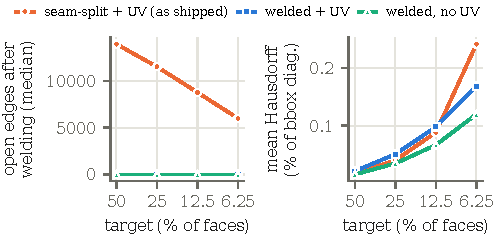
\includegraphics[width=\columnwidth]{figures/decimation}
\caption{Simplifying the 24 raw assets (medians). Left: boundary edges in the
output, counted after welding identical positions; the inputs have none.
Seam-split input cracks at every target; welded input, with or without UVs,
never does (the two lines coincide at zero). Right: mean surface distance to
the original.}
\Description{Two line charts over four simplification targets. Left: the
seam-split line falls from about 14,000 to 6,000 boundary edges; the welded lines
stay at zero. Right: mean distance rises for all three inputs, from about 0.02 to
0.24 percent of the bounding-box diagonal.}
\label{fig:decimation}
\end{figure}

\begin{table}[t]
\caption{Simplification at 6.25\,\% of the triangles (24 assets, up to three
passes). Distance: mean surface distance, \% of the bounding-box diagonal,
median [max]. Colour: base-colour RMSE above the unsimplified noise floor
(0--255 scale), median [max]. The maxima for W both come from the asset that
stalled. $^{*}$Normal preservation on; with it off, as for S and W, all 24 also
reach the target with no cracks.}
\label{tab:decimation}
\small
\begin{tabularx}{\columnwidth}{@{}Yrrrr@{}}
\toprule
Input & Reached & Cracked & Distance & Colour \\
\midrule
S: seam-split + UV & 18 & 24 & 0.24 [0.32] & 3.5 [9.6] \\
S, boundary preserved & 0 & 0 & -- & 2.4 [16.7] \\
W: welded + UV & 23 & 0 & 0.17 [1.40] & 3.7 [37.1] \\
N: welded, no UV$^{*}$ & 24 & 0 & 0.12 [0.20] & -- \\
\bottomrule
\end{tabularx}
\end{table}

H4 is not supported. Welded and with UVs preserved, 23 of 24 assets reached
6.25\,\% of their triangles (about 3,100) in one pass with no cracks
(Table~\ref{tab:decimation}). The exception has the most UV charts (3,088) and
stalled at 3,800--3,900 triangles after three passes (two runs). Charts constrain where the
simplifier may collapse, but at these budgets they rarely stop it.

What decided the outcome was the input. MeshLab's glTF loader returns the
file's seam-split buffer, in which every UV seam already separates the surface
into distinct vertices, as glTF requires~\cite{khronos2021gltf}. MeshLab's
texture-aware simplification then treats each seam as an open boundary. With
boundary preservation off (the default) the two sides of every seam move
independently: every asset cracked at every target, with a median of 13,924 open
edges already at 50\,\% (Figure~\ref{fig:decimation}), and six assets did not
reach 6.25\,\% within three passes. With boundary preservation on, nothing cracks
but nothing gets far: no asset went below 13,238 triangles, and the median stopped
at 21,939, about 44\,\% of the original. The filter reports no error in either
case. The failure depends on the tool. meshoptimizer, which infers seams from
matching positions~\cite{meshopt}, did not crack the same seam-split inputs but
stalled: two of 24 reached 6.25\,\% (median 5,900 triangles), against 24 of 24 on
welded input.

Welding identical positions first removes the problem in both tools; in
PyMeshLab this is one call, \texttt{meshing\_remove\_\allowbreak duplicate\_\allowbreak vertices},
which keeps UVs per corner. The
cost in colour is modest: median base-colour error above the noise floor is
1.5 levels at 12.5\,\% (0.1 for seam-split input) and 3.7 at 6.25\,\% (3.5), on a
0--255 scale, with one outlier at 37 for the asset that stalled. Mean surface
distance is slightly higher than for seam-split input at 50--12.5\,\% and lower at
6.25\,\%. Attribute discontinuities are a classic concern in
simplification~\cite{hoppe1996pm,hoppe1999newqem}, and the weld-first rule is
documented~\cite{meshopt}; what this case shows is how silently a common scripted
path runs into them.

This is what happened to the companion. Our pipeline loaded the 497,850-triangle
GLB directly and simplified it in three passes to 82,829 triangles, giving the
torn mesh of Section~\ref{sec:hygiene} (Figure~\ref{fig:assets}, bottom). The
design note for that step says the simplifier stopped near 106k triangles
because the UV islands were a hard floor. That figure came from an earlier trial
run; the shipped script multiplies the target by 0.55 per pass and simply ran its
three passes ($497{,}850 \times 0.55^3 \approx 82{,}830$). On the welded input the
same filter takes the companion to 31,116 triangles (6.25\,\%) in one pass with
no boundary edges. The torn mesh shipped after a play check recorded only as
``Play-verified'' in the commit history.


\subsection{History: three of six asset fixes repaired our own processing}
\label{sec:history}

Of 484 non-merge commits, 156 matched the pattern. After review they split into
61 \texttt{LEVEL}, 76 \texttt{OTHER}, 6 \texttt{ENGINE} and 13 \texttt{ASSET}.
Generated assets were a small part of the game's spatial trouble: level geometry,
purchased packs and procedural environment account for nearly five times as many
commits.

Seven of the 13 \texttt{ASSET} commits are not fixes but tooling written ahead of
need: the NPC import tool (scale to 1.7\,m, turn 180\textdegree, convert
material), its application to each era's models, the boss bake tool and the
companion's simplification and pivot setup. For the 24 static assets, scale and
pivot never became bugs: the developer noted them on the first imported file and
built the correction into the import step. The six fixes are a different list. Two repaired facing
(the $-Z$ front, then a second 180\textdegree{} turn that cancelled the first);
two repaired the companion lying on its back after our GLB-to-OBJ conversion
dropped the root rotation node; one was the boss hovering above its platform; one
was a scale calibration for the same problem. By origin, three were shipped by
the generator and three were introduced by our own processing (the double turn
and the lost rotation node, twice). Only three of the six concern a property a
metadata count would reveal, so H5 is not supported: facing (two fixes) is
invisible to counting, and grounding (the longest chain of fixes) needed the
animation to be evaluated.

\subsection{Grounding: the bind pose lies, and any constant has a floor}
\label{sec:grounding}

\begin{figure}[t]
\centering
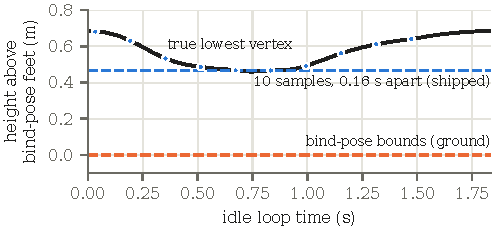
\includegraphics[width=\columnwidth]{figures/grounding_idle}
\caption{Boss idle loop at game scale (10\,m). Placing the bind-pose bounds on
the ground leaves the animated feet 0.46--0.68\,m in the air for the whole loop.
The shipped estimator (minimum of ten samples) lands within 6\,mm of the loop's
true minimum; the remaining 0.22\,m is the idle bob itself.}
\label{fig:grounding}
\end{figure}

The boss's studio mesh is skinned so that its bind pose stands with its feet at
the origin, but its idle animation lifts the whole body (Figure~\ref{fig:grounding}).
Snapping the bind-pose bounds to the ground, the engine's default and the game's
first attempt, leaves the animated feet 0.46--0.68\,m above the platform on every
frame. A single sampled frame can land anywhere in the 0.22\,m bob. The shipped
estimator, the minimum of ten samples 0.16\,s apart, reaches the loop's minimum
to within 6\,mm in Blender. What remains is not estimator error: a model moved by
one constant offset cannot follow a body that moves up and down, so 0.22\,m of
hover at the top of each bob is the floor for any constant, and only per-frame
contact handling (foot IK~\cite{kovar2002footskate}) goes below it. In the engine
the same estimator needed a further empirical 0.30\,m because Unity's
\texttt{BakeMesh} returned two incompatible scalings for this rig (0.68 and 2.29
against a hover of about 0.9 bracketed in play); we report those figures from the
commit record and did not reproduce them.
